\section{Ruby on Rails} % (fold)
\label{solution:sec:ruby_on_rails}
The main focus related with Ruby on Rails itself was to improve the current tools for profiling and benchmarking applications. Motivating the adoption of the soon to be released version of this framework---Rails 3---by the community was also a goal regarding this component. Increasing the community's awareness of this subject was also addressed by publishing an article to a popular magazine and engaging in a summer project---Ruby Summer of Code---with high visibility. Nonetheless, some common pitfalls were also addressed while presenting and benchmarking their solutions.

Improving Rails' profiling tools, motivating the adoption of Rails 3 and increasing the community's awareness of this subject were the general goals of the work presented in this section.


\subsection{Benchmarking}
Rails developers can often incur in some development performance pitfalls which can easily be addressed by using some of Rails' powerful functionalities. This section will cover some of these possible pitfalls, propose solutions and generally assert their performance differences.


\subsubsection{Eager Loading}
Eager loading is a core feature of Ruby on Rails which, in certain situations, can lead to significant performance slowdowns because of its absence or misuse. It allows the developer to specify if and which associations should be loaded up front, being the opposite of lazy loading. A classical example of the usefulness of this feature consists in a blog post with comments in which rendering the post's page will also render its comments. Eager loading allows the developer to specify that the comments should be loaded alongside the post, instructing Rails to only use two database queries---one for the post and another for its comments. If not explicitly specified, Rails will load each comment independently while rendering them. Loading the post and eager loading its comments is illustrated in the following code.
\begin{lstlisting}[xleftmargin=30pt,xrightmargin=30pt]
@posts = Post.find(:all, :include => :comments)
\end{lstlisting}

A simple benchmark was performed on a scaffold blog Rails application. The Rails version in use was 2.3.5. The database in use was MySQL using Ruby's default library. A thousand blog posts were generated automatically, along with two hundred thousand comments randomly associated with blog posts. This benchmark compares the time needed to complete a request which fetches all posts along with their comments. The test was run five times to eliminate circumstantial issues and the best results are shown. The results are exhibited on table~\ref{tab:eager_loading}.
\begin{table}[h!t]
  \centering
  \caption{Eager Loading Benchmark Results}
  \label{tab:eager_loading}
  
  \begin{tabular}{c|c}
  
    \textbf{\textsc{Eager Loading}} & \textbf{\textsc{Time (seconds)}} \\
    \hline
    No & 283 \\ \hline
    Yes & 21 \\
  \end{tabular}
\end{table}

In this extreme example, eager loading the data took $\pm$7\% of the time needed to lazy load the data, which is Rails default behavior. Eager loading can have a significant performance impact, depending on the context, as exemplified.


\subsubsection{Transactions}
Rails wraps every database write and update inside a transaction if not instructed otherwise. This happens because of its before/after filter functionality, which allows developers to hook code before and after certain actions are executed. In these cases, the operation and its filters are wrapped inside a transaction.

There are cases, however, where this behavior is suboptimal. When write/update calls are being executed consecutively---for instance, inside a loop---all database calls will be inside their own transaction. This will incur in significant performance penalties, depending on the amount of database actions. However, Rails allows developers to specify where the transaction should begin and end. The following code exemplifies this statement.
\begin{lstlisting}[xleftmargin=30pt,xrightmargin=30pt]
ActiveRecord::Base.transaction do
  (1..100).each { |i| Number.create(:value => i) }
end
\end{lstlisting}
In this example, instead of using one hundred transactions Rails will only use a single one. Using the same environment from the benchmark in the previous section, a benchmark was conducted on asserting the performance difference in explicitly using a global transaction instead of letting Rails place many small transactions which is, as previously mentioned, its behavior by default. This benchmark consisted in creating posts and associated comments, all with the same content. Two tests were made, the first by creating one hundred posts with twenty comments each and a second one by creating one post with two comments. Results can be seen on table~\ref{tab:transaction}.
\begin{table}[h!t]
  \centering
  \caption{Explicit Transaction Benchmark Results}
  \label{tab:transaction}
  
  \begin{tabular}{c|c|c}
  
    & \textbf{\textsc{Explicit Transaction}} & \textbf{\textsc{Time (milliseconds)}} \\ \hline
    100 posts, 20 comments & No & 76017 \\ \hline
    100 posts, 20 comments & Yes & 5223 \\ \hline
    1 post, 2 comments & No & 176 \\ \hline
    1 post, 2 comments & Yes & 137 \\
  \end{tabular}
\end{table}

Using a global transaction on the heaviest test implied a $\pm$93\% reduction on the time needed to write the data. On the lighter test, however, this reduction was of $\pm$22\%. On consecutive writes and/or updates, using a global transaction can significantly increase the performance of the operation.


\subsubsection{Magic Finders}
Rails has a feature commonly called ``magic finders''. It improves code's readability by allowing the developer to replace some calls with smaller and more readable ones. The following example illustrates this feature, comparing with a regular call.\\\\\\ % FIXME: next page?
\begin{lstlisting}[xleftmargin=30pt,xrightmargin=30pt]
Comment.find(:first, :conditions => ["created_at = ?", "2009-11-06 18:25:48"]) # normal find

Comment.find_by_created_at("2009-11-06 18:25:48") # magic find
\end{lstlisting}
These calls, however, have an associated performance penalty. Using the same test environment found on the previous benchmarks, both previously presented calls were benchmarked. The results are presented on table~\ref{tab:magic_finders}.
\begin{table}[h!t]
  \centering
  \caption{Magic Finders Benchmark Results}
  \label{tab:magic_finders}
  
  \begin{tabular}{c|c}
  
    \textbf{\textsc{Type}} & \textbf{\textsc{Time (milliseconds)}} \\ \hline
    Normal find & 62 \\ \hline
    Magic find & 197 \\
  \end{tabular}
\end{table}

The normal find only takes $\pm$32\% of the time needed by the magic find to complete. Since there is a readability/performance trade-off, using either syntaxes is a decision which depends on the project and its developers. The general performance penalty associated with the commonly used magic finders is, however, significant and should be taken into account.


\subsubsection{Fetching Large Groups of Records}
In certain situations, Rails applications need to fetch a significant amount of rows from the database, instantiate each model object and render them in a view. Using the ``find'' helper, this operation can be significantly heavy on memory, as it fetches and loads all records into Ruby objects, and will lock the application until all operations are complete.

However, when Rails 2.3 was introduced it bundled a couple of methods which are likely to be very useful in these situations: ``find\_each'' and ``find\_in\_batches''. The first will retrieve a specified amount of objects at a time, letting the code iterate over the records as if it was a normal ``find'' call. The second is very similar, except that it gives control back to the application every time it fetches a batch. Both methods have a ``batch\_size'' option which defaults to one thousand records. These additional methods have the advantage of using less memory and, as explored in Section~\ref{state:sec:ruby}, less memory usage will trigger Ruby's garbage collector less often, providing better execution times. Notwithstanding these advantages, these methods are unlikely to yield performance improvements when fetching small amounts of records.

To accurately determine the performance benefits involved with switching the ``find'' call with ``find\_each'' when there is a significant amount of records involved, a benchmark was done. The environment was the same as previous benchmarks. The test itself consisted in fetching the two hundred thousand comments in the example blog application. The results can be found on table~\ref{tab:fetch_in_batches}.
\begin{table}[h!t]
  \centering
  \caption{Fetching Records in Batches Benchmark Results}
  \label{tab:fetch_in_batches}
  
  \begin{tabular}{c|c|c}
  
    \textbf{\textsc{Method}} & \textbf{\textsc{Time (seconds)}} & \textbf{\textsc{Memory Usage (MB)}} \\ \hline
    find & 211 & 158 \\ \hline
    find\_each & 195 & 118 \\
  \end{tabular}
\end{table}

Using the alternative method to fetch records in batches, the application needed 10\% less time to fetch the records and used 25\% less memory. These are significant improvements, mainly in memory usage.

\subsection{Development}
The development phase regarding this component involved many distinct activities. First of all, it was crucial to refactor Rails' native profiling and benchmarking tools. Taking into consideration that the release of the new version of the Ruby on Rails framework is nearing, it was important to motivate its early adoption by porting some widely used plugins/gems and one of this framework's most famous applications to the most recent version. After that, a small task related to adding support for the Nginx's \textit{X-Accel-Redirect} header to Rails was performed. Finally, an overview on the current work under the Ruby Summer of Code program is given.


\subsubsection{Refactoring Rails Profiling/Benchmarking Tools}
Rails' profiling and benchmarking tools were nonfunctional on YARV, as they relied on Rub 1.8's now outdated architecture. Ruby evolved very fast and these tools did not keep up, becoming deprecated and useless when used on this version.

Adding Ruby 1.9  support to these tools was crucial, since developers could not rely on the native tools when benchmarking and profiling their applications. By taking advantage of the enhances made to Ruby's profiling tools mentioned in Section~\ref{solution:sec:ruby}, Rails was overhauled~\footnote{\url{http://github.com/rails/rails/commits/master?author=goncalossilva}} and now fully supports profiling and benchmarking under Ruby 1.9.


\subsubsection{Porting Plugins to Rails 3}
Rails 3 adoption by developers is highly conditioned by plugin availability. As mentioned in Section~\ref{tech:sec:ruby_on_rails}, there is a significant amount of plugins available for Ruby on Rails. However, due to the recent Rails' architectural changes, authors generally need to update their plugins/gems to be compatible to this version. The lack of available plugins will certainly limit the adoption rate of this version. In order to help alleviating this problem, some famous plugins were updated to comply with the new Rails API for plugins/gems. All plugins used by \textit{Escolinhas.pt} were analyzed and the ones with the higher watcher count\footnote{GitHub allows users to start ``watching'' repositories, being notified of all changes made to the projects they ``watch''} on their public repositories, were selected. Their names and functionality are:
\begin{description}
  \item[acts\_as\_list,] a plugin for sorting and reordering a number of objects in a list\footnote{\url{http://github.com/goncalossilva/acts_as_list/}};
  \item[permalink\_fu,] a plugin for creating URL-friendly permanent links from object attributes\footnote{\url{http://github.com/goncalossilva/permalink_fu/}};
  \item[acts\_as\_paranoid,] a plugin for hiding records instead of deleting them, being able to recover them\footnote{\url{http://github.com/goncalossilva/rails3_acts_as_paranoid/}}.
\end{description}
All the mentioned plugins were refactored to use the new plugin API. Some tests also needed refactoring, as they used deprecated Rails code. However, updating \textit{permalink\_fu} also involved replacing its character conversion engine since it relied on deprecated Ruby 1.8 functionality, meaning this plugin was not compatible with Ruby's most recent version. On the other hand, \textit{acts\_as\_paranoid} had to be completely rewritten. It was initially developed for Rails 1 and slightly patched to work on Rails 2, having a deprecated architecture which was incompatible with Rails 3. Recreating this plugin from ground up with Rails 3 in mind allowed a $\pm$70\% reduction in lines of code.


\subsubsection{Porting Redmine to Rails 3}
Redmine\footnote{\url{http://www.redmine.org/}} is an open-source flexible project management web application written in Ruby on Rails, created by Jean-Philippe Lang. It is one of the most famous open-source Rails projects, having more than 90 reported major installations worldwide~\cite{redmine_installations}, including the development teams of Ruby, phpBB and Lighttpd. It is a complex platform with over 60 models and 65000 lines of code.

Redmine was upgraded to use Rails 3 and the source code is at GitHub\footnote{\url{http://github.com/goncalossilva/redmine}}. This upgrade increased Rails 3's visibility while showing the potential performance improvements in upgrading, since this version is reportedly faster. The benefits can be experienced by the users themselves while using Redmine. Many issues had to be addressed, including fixes on the application initialization process, string handling, parameter filtering, plugin support, usage of Javascript helpers and method overriding, among others. All changes can be explored in detail on the project's commit log at GitHub.


\subsubsection{Adding X-Accel-Redirect Support to Rails}
Rails lacks support for Nginx's \textit{X-Accel-Redirect} header by default, so a plugin to add it was developed\footnote{\url{http://github.com/goncalossilva/X-Accel-Redirect}}. Similar to Apache's \textit{X-Sendfile}, \textit{X-Accel-Redirect} can be useful when a user requests the download of a file from the server. If this flag is set on the response body, it will instruct Nginx to handle the file delivery itself. This way, the Rails process will be free to handle other requests instead of blocking to serve the file, delegating that task to Nginx.


\subsubsection{Benchmarking Continuous Integration}
Late in this project's course, applications for the Ruby Summer of Code\footnote{\url{http://www.rubysoc.org/}} began. This program is similar to Google Summer of Code, being a student internship program designed to help fund student development of Ruby-related projects during the summer.

The decision to apply for this program was made, by proposing the development of a Benchmarking Continuous Integration for Ruby on Rails. This proposal was later accepted and a project mentor assigned---Yehuda Katz. Yehuda, the lead developer of the discontinued Merb framework, is one of the most prominent developers behind Rails 3, having joined the core team as soon as the decision to merge Rails and Merb became official.

``Project \#8: Benchmarking CI\footnote{\url{http://www.rubysoc.org/projects/}}'' consists in building an official full-stack benchmarking suite for Ruby on Rails. This way, each commit to the Rails repository will automatically trigger a process where a remote machine starts a new server, runs the tests and reports back the results. As time goes by, it will be possible to watch the evolution of the framework's performance and developers will be able to keep track of the impact their changes have. Any performance regressions will be detected and the responsible developers notified. In its most basic form, it will bring a kind of performance-oriented continuous integration for the Ruby on Rails framework.

The whole Rails community will benefit from having an official benchmarking suite for Ruby on Rails. On one hand, developers will have increased awareness of the framework's performance. They will be able to benchmark their changes and understand their impact on every component, making small adjustments if any significant performance regressions are found. On the other hand, the community will also benefit since Rails will definitely become faster and more scalable over time.


\subsection{Community Blog}
Soon after the start of the project, a public blog named ``Snap Rails''\footnote{\url{http://snaprails.tumblr.com}} was created. Many of the findings done throughout this project have been presented there. Despite being fairly recent, it already surpasses a thousand unique visitors. A map overlay showing their locations is shown on figure~\ref{fig:snaprails_map_overlay}.
\begin{figure}[h!t]
  \centering
    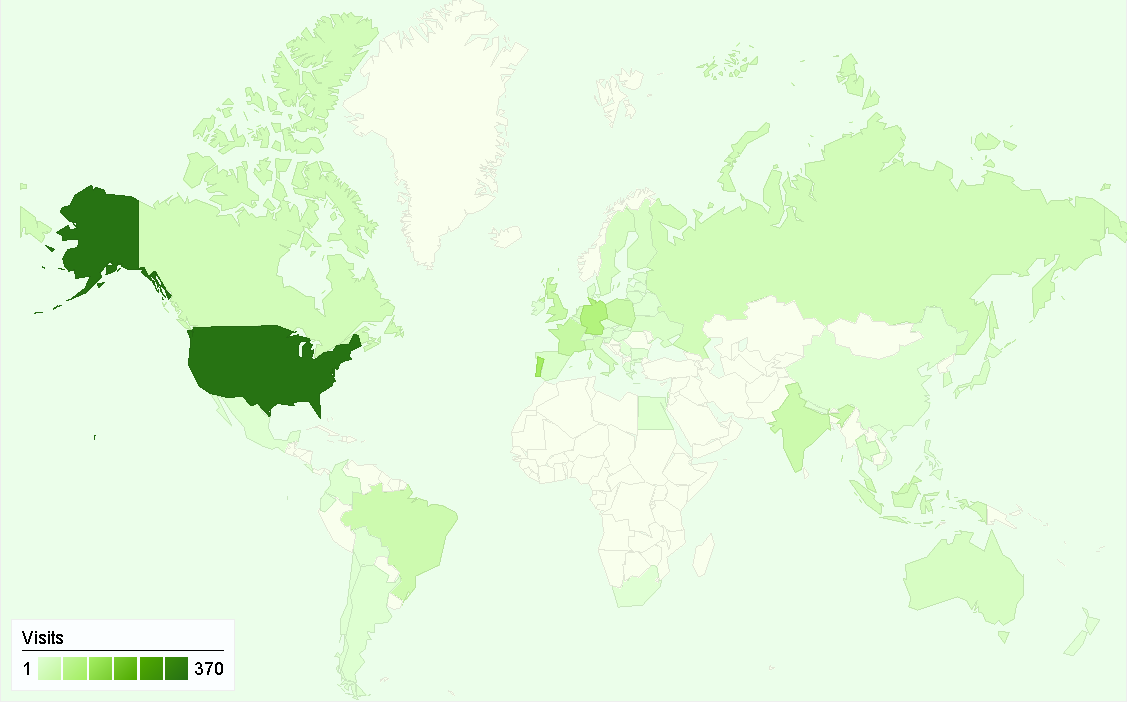
\includegraphics[width=0.75\textwidth]{snaprails_map_overlay}
    \caption{``Snap Rails'' Map Overlay} \label{fig:snaprails_map_overlay}
\end{figure}
Visitor analysis was made using Google Analytics\footnote{\url{http://analytics.google.com}}. With visitors from more than fifty five countries, this blog's purpose is to continuously increase this subject's visibility.


\subsection{Performance-oriented Article Series}
A series of performance-oriented articles for the \textit{Rails Magazine} has also begun. The first article is already present on the sixth edition of the magazine~\cite{rails_magazine_6}, with more to follow on future releases. Similarly to this thesis, this article performance series will cover all system's components, having already started with an introduction to this subject. A copy is exhibited in appendix~\ref{ap:rails_magazine}.

Publishing articles on this matter on such a popular magazine increases this subjects' visibility and the importance in building highly scalable Ruby on Rails applications, possibly igniting the community's awareness of this subject.


\subsection{Section Overview}
This section exhibited and explained the work concerning Ruby on Rails. Regarding benchmarking, common performance pitfalls and their solutions were analyzed. Concerning development, Rails' profiling and benchmarking tools were revamped and now seamlessly integrate with Ruby's. After that, some renowned plugins and Redmine were ported to Rails 3. A plugin which adds support for Nginx's \textit{X-Accel-Redirect} was also created. Finally, a project related to the creation of a performance-oriented continuous integration for Rails under the Ruby Summer of Code program was detailed. This section also presents some work that does not fit under the usual fields---benchmarking, development and tweaking---which is related with increasing the community's awareness of the importance of building highly performant Rails applications. This work is related with the creation of a community blog on this subject and the start of a performance-oriented series of articles for \textit{Rails Magazine}.

Making Rails' profiling tools agnostic to which Ruby version is using them and consequently seamless integrate with YARV allowed to improve these tools. Porting Redmine and various plugins to Rails 3 increased this version's visibility and eased the process of upgrading, motivating its adoption. Creating the general guidelines by using information from this and previous sections, starting a community blog and writing an article series are likely to increase the community's awareness of this subject. Finally, building a benchmarking continuous integration for Rails itself will also increase its developer's awareness of this subject, completing the last of the general goals initially stated.
